\section{Requirement 3: highly non-stationary multiple-campaigns environment}

% ============================================================
% Overview
% ============================================================
\begin{frame}{Highly non-stationary multiple-campaigns environment}
    \begin{itemize}
        \item Sequence of highest competing bids $(m_t^{(i)})_t$ sampled from a distribution that \emph{changes quickly and continuously over time}
        \item Different patterns per campaign but possibly \emph{correlated} through market regimes (e.g., holidays, Black Friday)
        \item UCB-style methods break: confidence radius assumes stationarity
        \item Algorithm to be studied: \textbf{primal-dual} with budget, assuming full feedback
        \begin{itemize}
            \item Full-feedback: highest competing bid $m_t^{(i)}$ is observed, providing information about all arms regardless of which one we bid on
            
            $\implies$ a regret minimizer for the adversarial expert problem (\textbf{Hedge}) is appropriate!
        \end{itemize}
    \end{itemize}
\end{frame}

% ============================================================
% Distribution model
% ============================================================
\begin{frame}{Distribution model: adversarial-style sinusoids}
    \begin{columns}[T]
        \lfill\begin{column}{0.4\textwidth}
            \small\textbf{Modeling choice:}
            \begin{itemize}
                \item Each competitor's bid at round $t$ is drawn from $\mathrm{Unif}(0, u^{(i)}_t)$ where
                \begin{equation*}
                    \begin{aligned}
                        u^{(i)}_t &= low^{(i)} + \\ 
                        & (high^{(i)} - low^{(i)})\bigl(1 - |\sin(5t/T)|\bigr)
                    \end{aligned}
                \end{equation*}
            \end{itemize}
        \end{column}
        \begin{column}{0.45\textwidth}
            \centering
            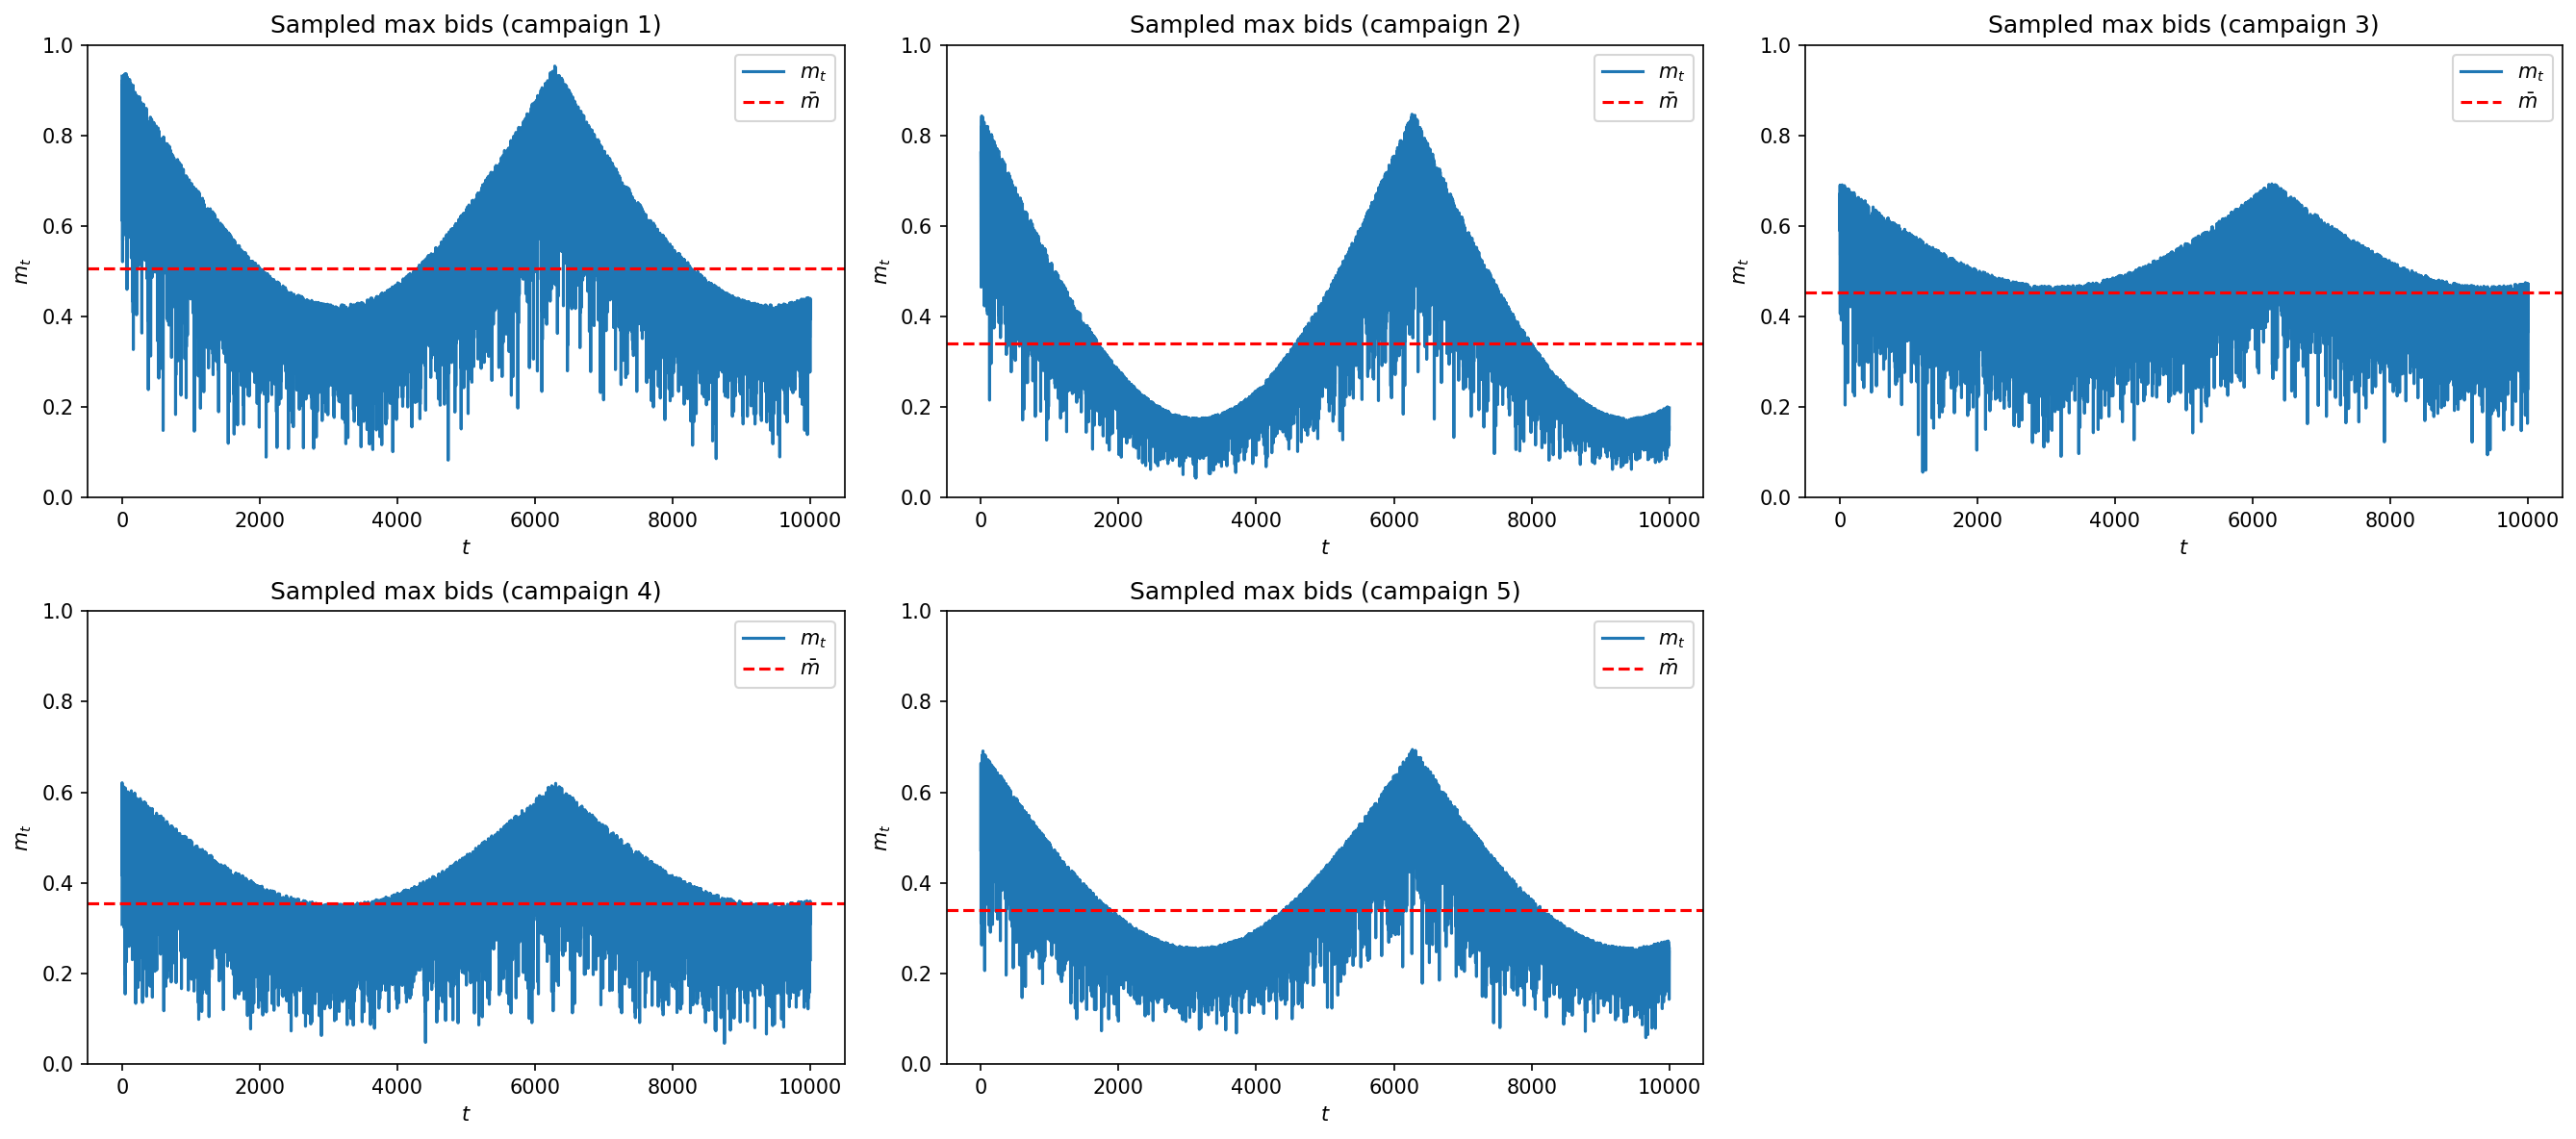
\includegraphics[width=\textwidth]{figures/req3_max_bids_ts.png}
        \end{column}
    \end{columns} 

    \vspace{0.1cm}

    \small\begin{itemize}
        \item Same frequency across campaigns: models price changes due to the \emph{shared market conditions}, like sales (Black Friday), holidays (Christmas), \ldots during which showing ads is more valuable and competitors are likely to bid more
        \item $high$ and $low$ represent the range of the oscillations
        \item Max of uniforms is Beta-distributed \emph{within each round}, but the parameters change continuously, so the Beta distribution is actually rescaled
    \end{itemize}
\end{frame}

% ============================================================
% Clairvoyant LP - highly non-stationary
% ============================================================
\begin{frame}{Clairvoyant}
    \begin{itemize}
        \item We want to use a similar LP to that of the clairvoyant for Requirement 2
        \item The previous clairvoyants used the true win probabilities $\mathbb{P}\left[ m \le b \right]$ from the known underlying stationary distribution 
        \item But: now, the distribution of the highest competing bids keeps changing quickly throughout the rounds $\implies$ no fixed win probabilities!
    \end{itemize}

Instead, use the estimates $\hat{\mathbb{P}}\left[ m \le b \right]$ of the empirical win probabilities (computed in hindsight)!
        
    \begin{block}{Assumption} 
        The clairvoyant knows the empirical win probability $\hat{\mathbb{P}}\left[ m \le b \right]$ a posteriori of each bid $b$ (like in the exercise session).
    \end{block}
\end{frame}

\begin{frame}{Clairvoyant: from Requirement 2 to Requirement 3}
    \vspace{-0.4cm}
    \footnotesize\begin{equation*}
        \begin{aligned}
            \gamma_s^\star, [\gamma_i]^\star = \arg & \max_{\gamma_s \in \mathbb{R}^{2^N}, [\gamma_{S, i}] \in \mathbb{R}^{NK}} ~~~ \sum_S \sum_{i \in S} \sum_b \gamma_{S, i}(b)\, \textcolor{red}{\bar{f}^{(i)}(b)} \\
            & \begin{aligned} 
                \text{s.t.} ~~~~~~~~~~~~~~~~~~ & \sum_S \sum_{i \in S} \sum_b \gamma_{S, i}(b)\, \textcolor{red}{\bar{c}^{(i)}(b)} \le \rho \quad & \text{(budget)} \\
                & \sum_S \gamma_s(S) = 1 & \text{(subset probability)} \\
                & \sum_b \gamma_{S, i}(b) = \gamma_S(S) \quad \forall S, i & \text{(marginalization)} \\
                & \gamma_{S, i}(0) = 0 \quad \forall S,\, \forall i \in S & \text{(campaign in subset)} \\
                &\gamma_{S, i}(0) = 1 \quad \forall S,\, \forall i \notin S & \text{(campaign not in subset)} \\
                & \gamma_s(S) = 0 \quad \forall S \text{ having conflicts} & \text{(conflict)} \\
                & 0 \le \gamma_s(S) \le 1 \quad \forall S \\
                & 0 \le \gamma_{S, i}(b) \le 1 \quad \forall b 
            \end{aligned}
        \end{aligned}
    \end{equation*}

    The win probabilities affect the LP from within $\textcolor{red}{\bar{f}^{(i)}(b)} = (v - b)\, \mathbb{P}_{m \sim \mathcal{D}_m}\left[ b \ge m \right]$ (and $\textcolor{red}{\bar{c}^{(i)}(b)}$): simply replace $\mathbb{P}_{m \sim \mathcal{D}_m}\left[ b \ge m \right]$ with $\hat{\mathbb{P}}_{m \sim \mathcal{D}_m}\left[ b \ge m \right]$!
\end{frame}

\begin{frame}{Clairvoyant: optimal $\gamma$ under highly non-stationarity}
    \centering
    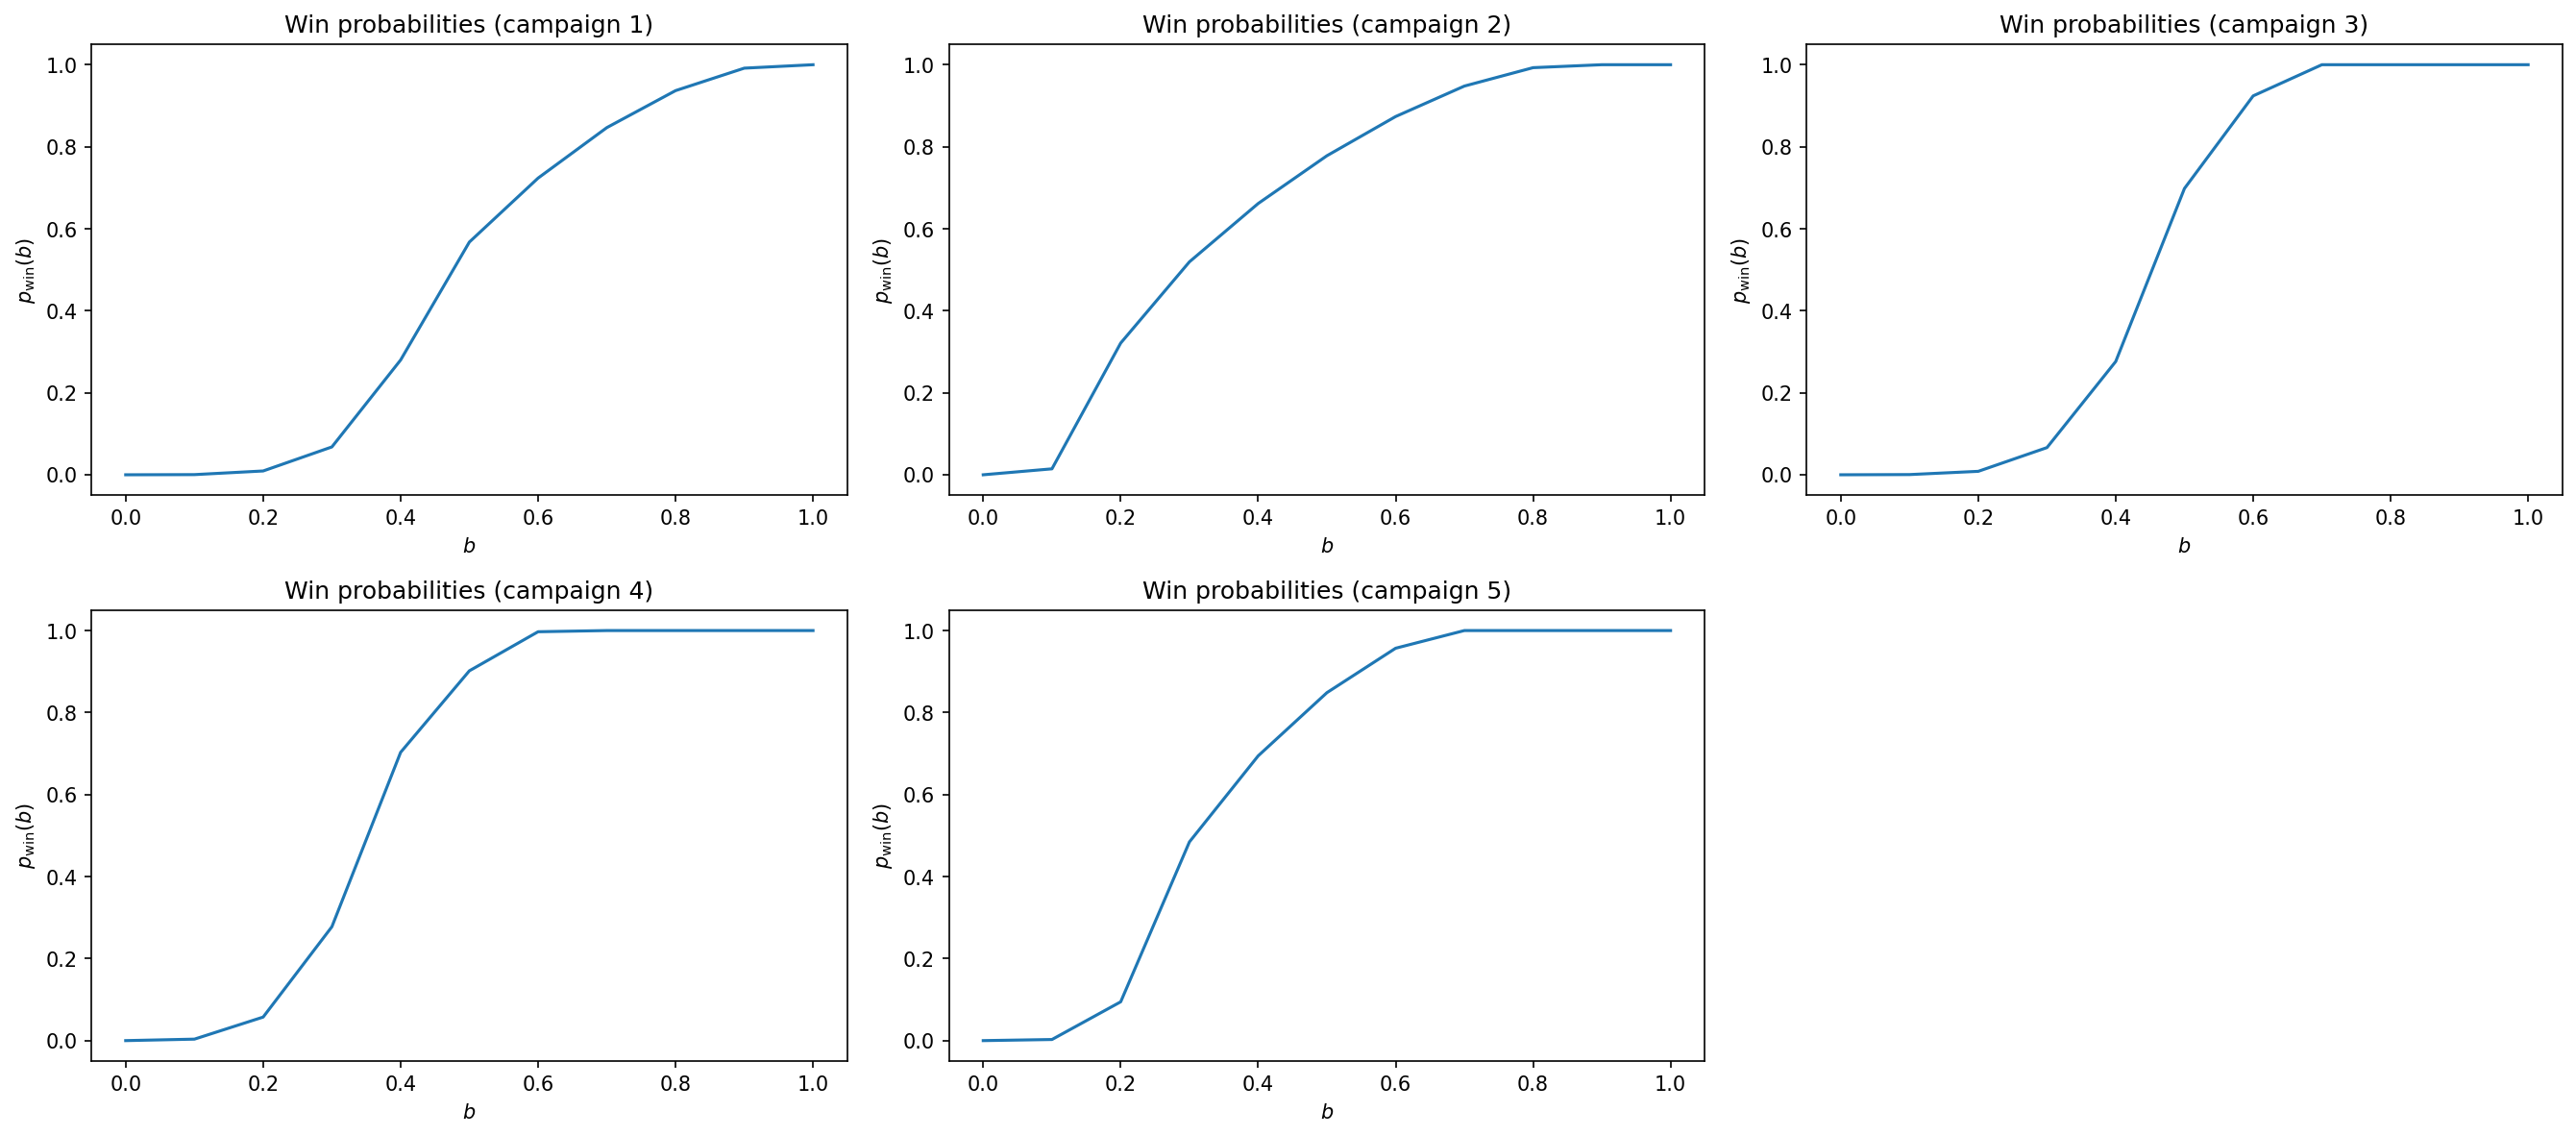
\includegraphics[width=0.5\textwidth]{figures/req3_win_probabilities.png}\hfill
    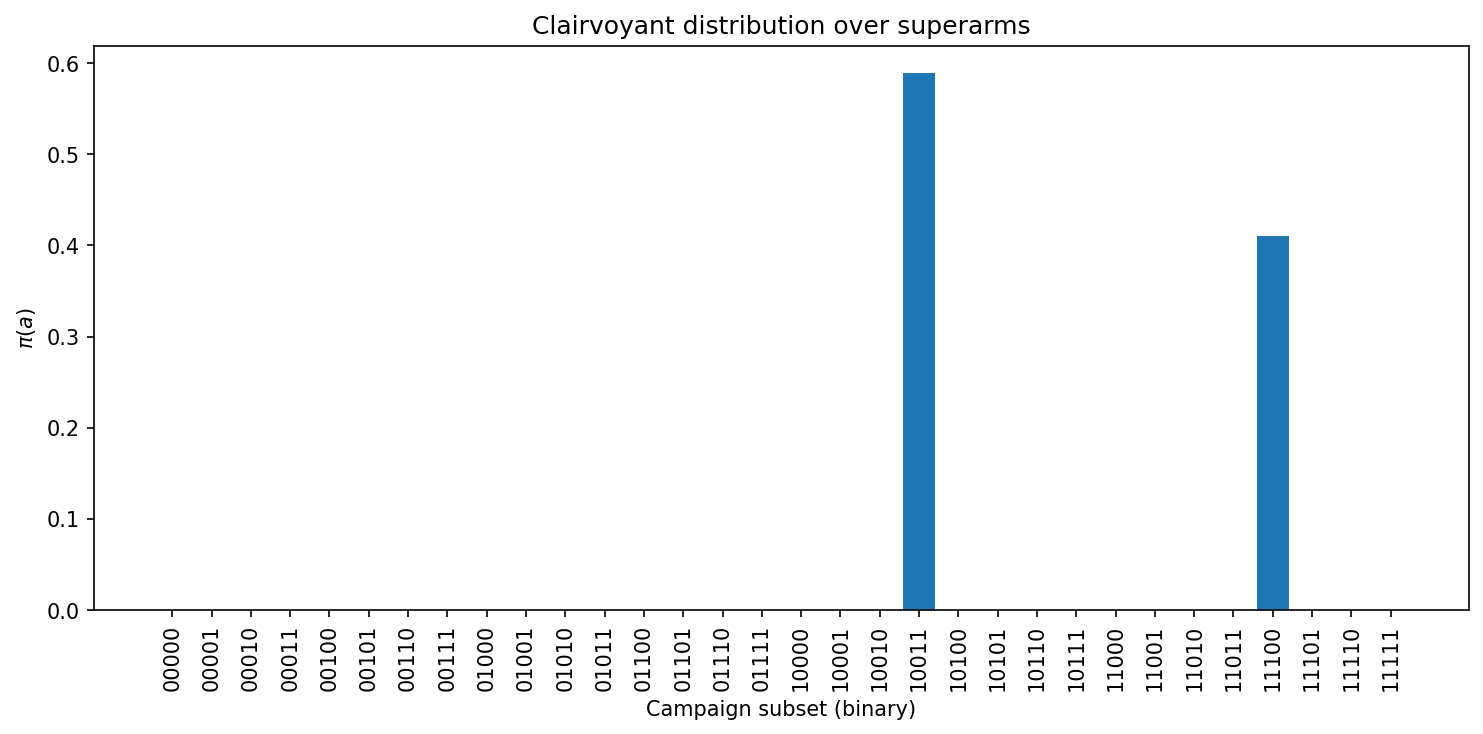
\includegraphics[width=0.48\textwidth]{figures/req3_clairvoyant_superarm.png}\\
    \scriptsize
    \textbf{Left:} empirical $\hat{\mathbb{P}}\left[b \ge m_t\right]$, estimated a posteriori over all rounds.\\
    \textbf{Right:} optimal strategy $\gamma^\star$ of the clairvoyant, which still randomizes over multiple campaigns subsets.
\end{frame}

% ============================================================
% Primal-Dual bidder
% ============================================================
\begin{frame}{Primal-dual bidder: optimization problem}
    \begin{block}{Remember:}
        $\gamma$ is the distribution over joint actions, induced in our case by the two-step sampling procedure
    \end{block}

    The optimization problem that we are solving is 
    \[\gamma^\star = \arg \max_{\gamma \in \Delta_\mathcal{B}} \bar{f}(\gamma) \qquad \text{s.t.  } \bar{c}(\gamma) \le \rho\]

    The probability simplex constraint is already enforced by the choice of Hedge as regret minimizer: the budget constraint is instead incorporated through the expected Lagrangian
    \[\bar{\mathcal{L}}(\gamma, \lambda) = \underbrace{\bar{f}(\gamma)}_{\text{expected utility}} - \lambda(\underbrace{\bar{c}(\gamma)}_{\text{expected payment}} - \rho)\]
    \vspace{0.2cm}
    where $\bar{f}(\gamma) = \sum_{i=1}^N \mathbb{E}_{\mathbf{b} \sim \gamma}\left[ \mathbb{E}_{(m^{(1)}, \cdots, m^{(N)}) \sim \mathcal{D_\mathbf{m}}}\left[ f^{(i)}(b_i, m_i) \right] \right]$ (and same for $\bar{c}(\gamma)$)
\end{frame}

\begin{frame}{Primal-dual bidder: structure}
    \begin{itemize}
        \item \textbf{Dual step (stochastic gradient ascent on $\lambda$):}
        \[\boxed{\lambda_{t+1} = \Pi_{[0,1/\rho]} \left(\lambda_t - \eta_d\,(\rho - c_t) \right)}\]

        in which $c_t$ is estimating $\bar{c}(\gamma)$ in the expected Lagrangian
    \end{itemize}
\end{frame}

\begin{frame}{Primal-dual bidder: structure}
    \begin{itemize}
        \item \textbf{Primal step (multiplicative Hedge updates on $\gamma$):} $N + 1$ separate Hedge instances on
        \begin{itemize}
            \item $N$ per-campaign bid distributions $\gamma_i$ over $\mathcal{B}\, \backslash\, \{0.0\} \rightarrow$ Hedge updates: \[w_{t+1}^{(i)}(b) = w_t^{(i)}(b)\, e^{-\eta_p \ell_t^{(i)}(b)} \quad \forall b \in \mathcal{B}\]
            \item campaigns-subsets distribution $\gamma_s$  $\rightarrow$ Hedge updates: \[w_{t+1}(S) = w_t(S)\, e^{-\eta_p \mathcal{L}_t(S)} \quad \forall S \in \mathcal{\mathcal{P}(N)}\]
        \end{itemize}
    \end{itemize}

    \begin{block}{}
        Same decomposition as the Combinatorial-UCB bidder in Requirement 2!
    \end{block}
    
    \begin{block}{}
        Conflicts are masked by initializing to $0$ the weights corresponding to invalid superarms: Hedge's multiplicative updates won't be able to change these weights
    \end{block}
\end{frame}

\begin{frame}{Primal-dual bidder: structure}
    \begin{itemize}
        \item \textbf{Primal step (multiplicative Hedge updates on $\gamma$):} 
        \[w_{t+1}^{(i)}(b) = w_t^{(i)}(b)\, e^{-\eta_p \textcolor{red}{\ell_t^{(i)}(b)}} \quad \forall b \in \mathcal{B}\]
        \[w_{t+1}(S) = w_t(S)\, e^{-\eta_p \textcolor{red}{\mathcal{L}_t(S)}} \quad \forall S \in \mathcal{\mathcal{P}(N)}\]

        \begin{block}{}
            We actually use two kinds of Lagrangians for the primal step: one "global" Lagrangian $\mathcal{L}_t$ (like the dual one) for Hedge over the campaigns subsets, and single-campaign Lagrangians $\ell_t$ for the Hedge instances over the single campaigns
        \end{block}
    \end{itemize}
\end{frame}

\begin{frame}{Primal-dual bidder: Lagrangians}
    At round $t$, we observe the highest competing bid $m_t^{(i)}$ for all bids in all campaigns:
    \begin{itemize}
        \item $f_t^{(i)}(b_i) = (v_i - b_i)\,\mathds{1}\left[ b_i \geq m_t^{(i)} \right]$ is the utility obtained from campaign $i$ if playing bid $b_i$
        \item $c_t^{(i)}(b_i) = b_i\,\mathds{1}\left[ b_i \geq m_t^{(i)} \right]$ is the payment for campaign $i$ if playing bid $b_i$
    \end{itemize}

    \vspace{1cm}

    The overall expected utility and payment for any subset $S$ of campaigns are
    \[f_t(S) = \sum_{i \in S} \mathbb{E}_{\mathbf{b} \sim \gamma_{i|S}}\left[ f_t^{(i)}(b_i) \right] = \sum_{i \in S} f_t^{(i)}(\gamma_{i|S}), \quad c_t(S) = \sum_{i \in S} \mathbb{E}_{\mathbf{b} \sim \gamma_{i|S}}\left[ c_t^{(i)}(b_i) \right] = \sum_{i \in S} c_t^{(i)}(\gamma_{i|S}).\]
\end{frame}

\begin{frame}{Primal-dual bidder: Lagrangians}
    With the budget constraint $c_t \leq \rho$, the global per-round Lagrangian is
    \[\boxed{\mathcal{L}_t(S, \lambda_t) = f_t(S) - \lambda_t(c_t(S) - \rho)}\]

    \vspace{-0.2cm}

    \begin{alertblock}{Key point}
        The term $\lambda_t\rho$ appears \textbf{once}, regardless of
        how many cammpaigns ($|S|$) are in subset $S$
    \end{alertblock}

    \vspace{0.2cm}

    The single-campaign Lagrangians, instead, only use $f_t^{(i)}(b_i)$ and $c_t^{(i)}(b_i)$ of one campaign:
    \[\boxed{\ell_t^{(i)}(b_i, \lambda_t) = f_t^{(i)}(b_i) - \lambda_t (c_t^{(i)}(b_i) - \rho)}\]
\end{frame}

% ============================================================
% Results: dual variable
% ============================================================
\begin{frame}{Results: dual variable $\lambda_t$ and per-round expense}
    \begin{columns}[T]
        \begin{column}{0.55\textwidth}
            \hfill
            \centering
            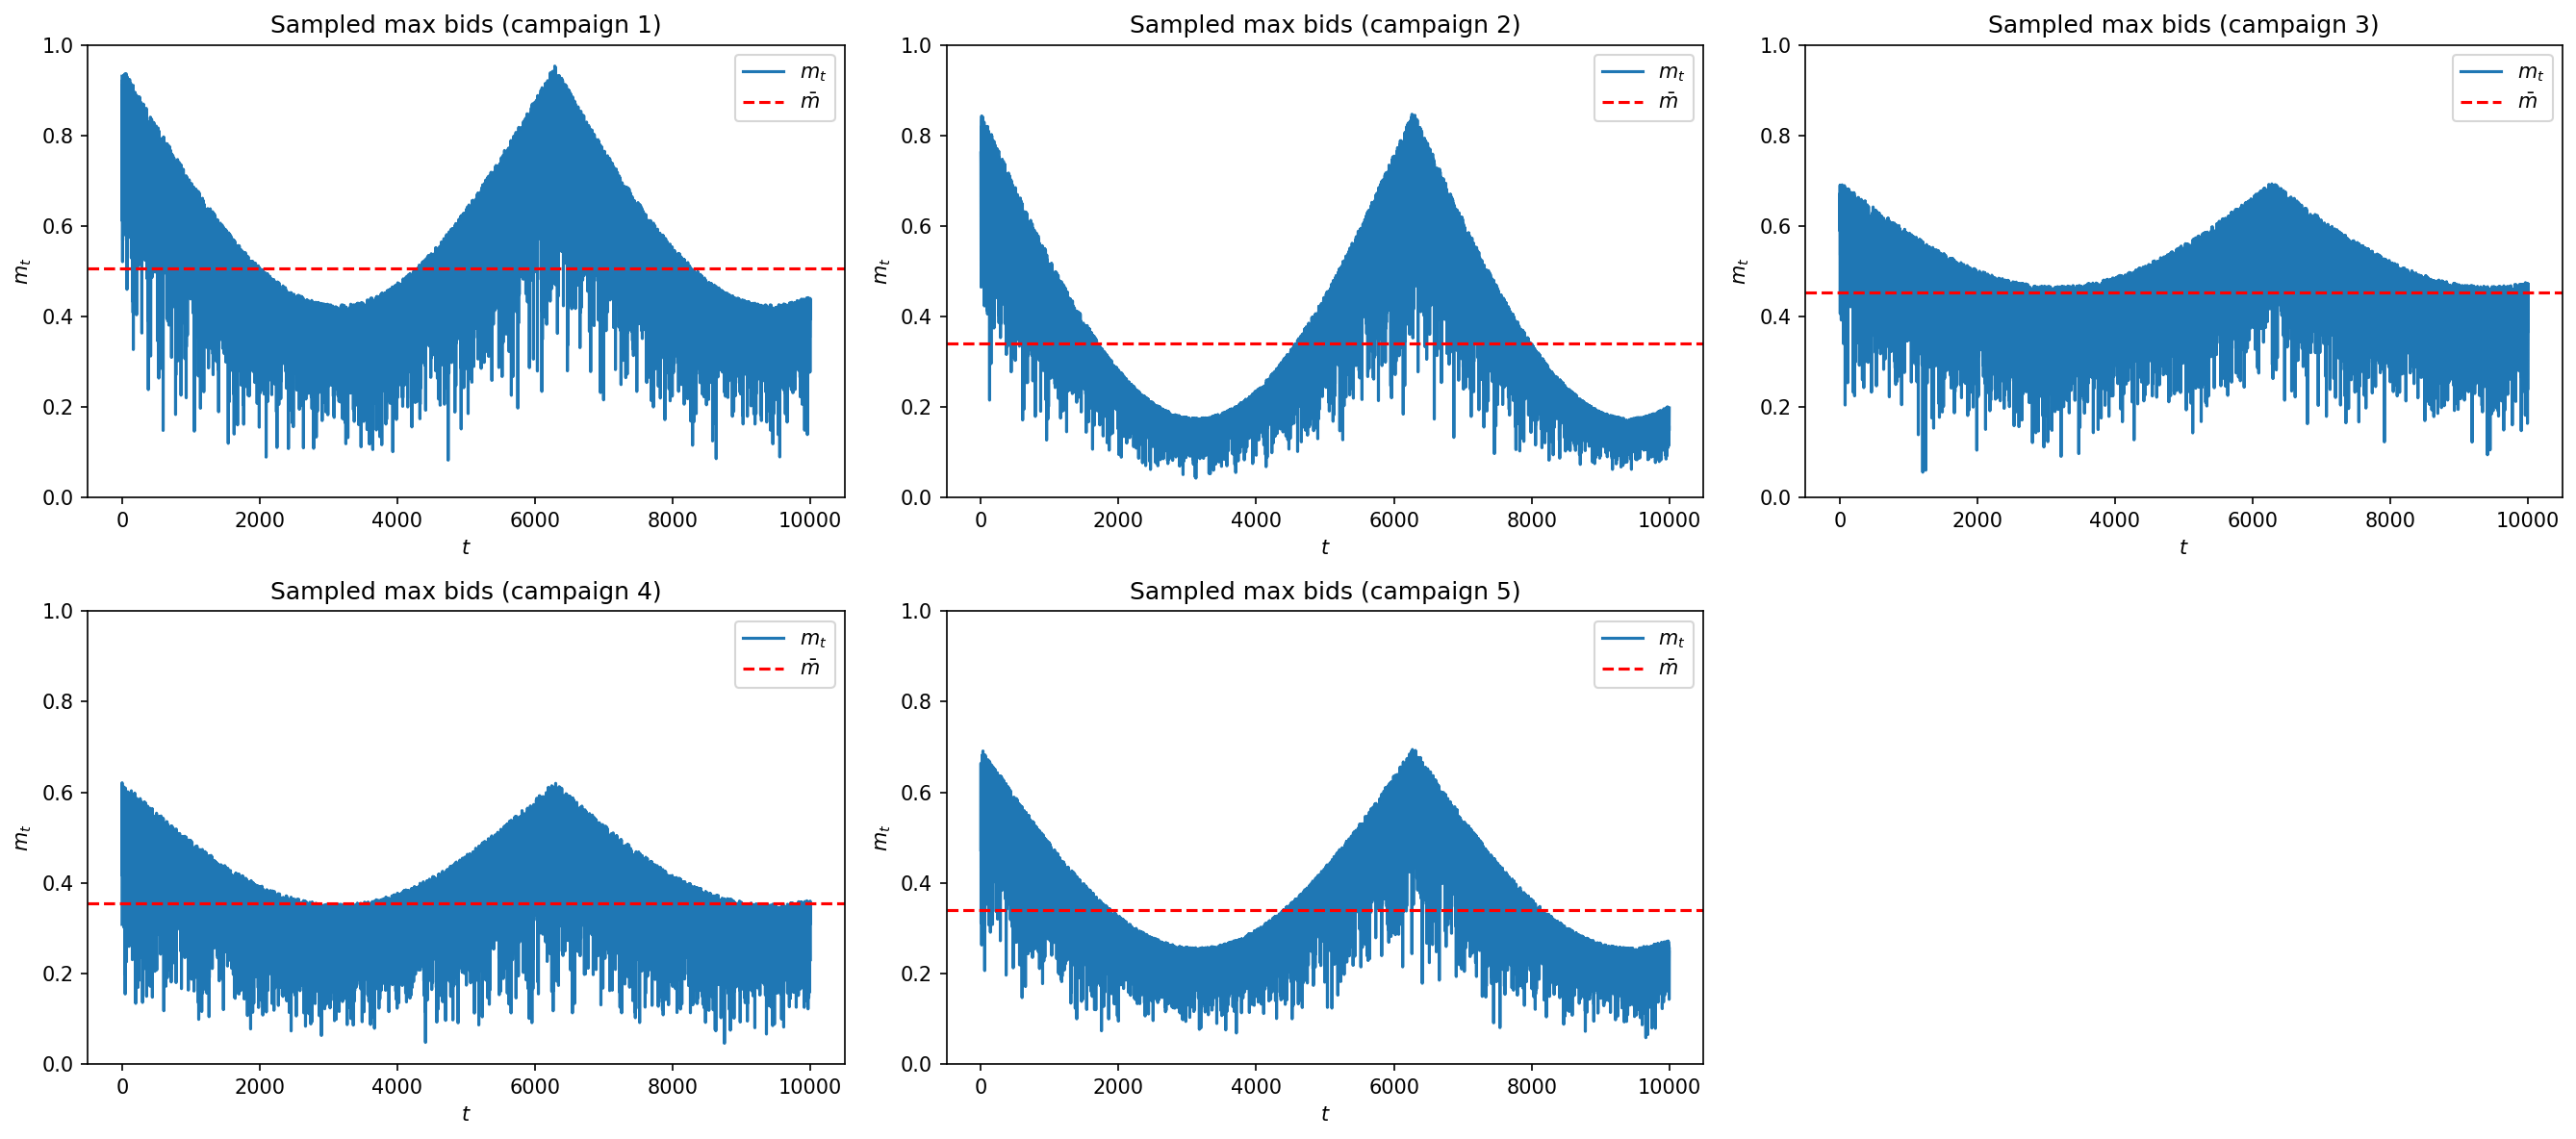
\includegraphics[width=0.95\textwidth]{figures/req3_max_bids_ts.png}\\
            \scriptsize
            $\lambda_t$ drifts upward or downward (\textbf{right: top plot}) respectively when the bidder spends less or more than $\rho$ (\textbf{right: bottom plot}). 
            \begin{itemize}
                \item During the peaks in the \textbf{left plot}, $\lambda_t$ decreases, counteracting the need of spending more due to the overall higher competing bids;
                \item during the valleys, lambda grows, because the current auctions being less expensive means that we could try to win them more often.
            \end{itemize} 
        \end{column}
        \begin{column}{0.35\textwidth}
            \centering
            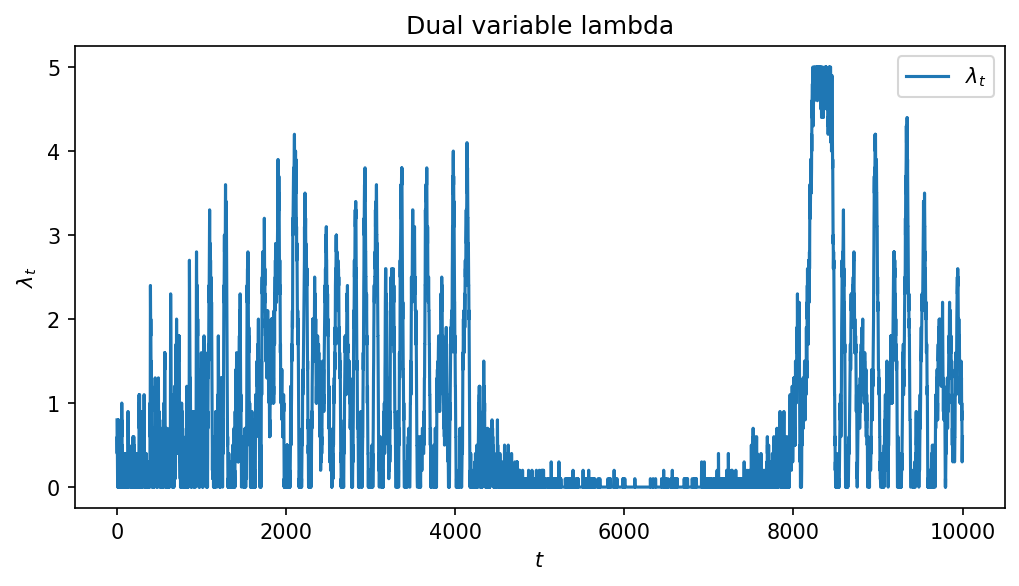
\includegraphics[width=1.1\textwidth]{figures/req3_dual_lambda.png}\\
            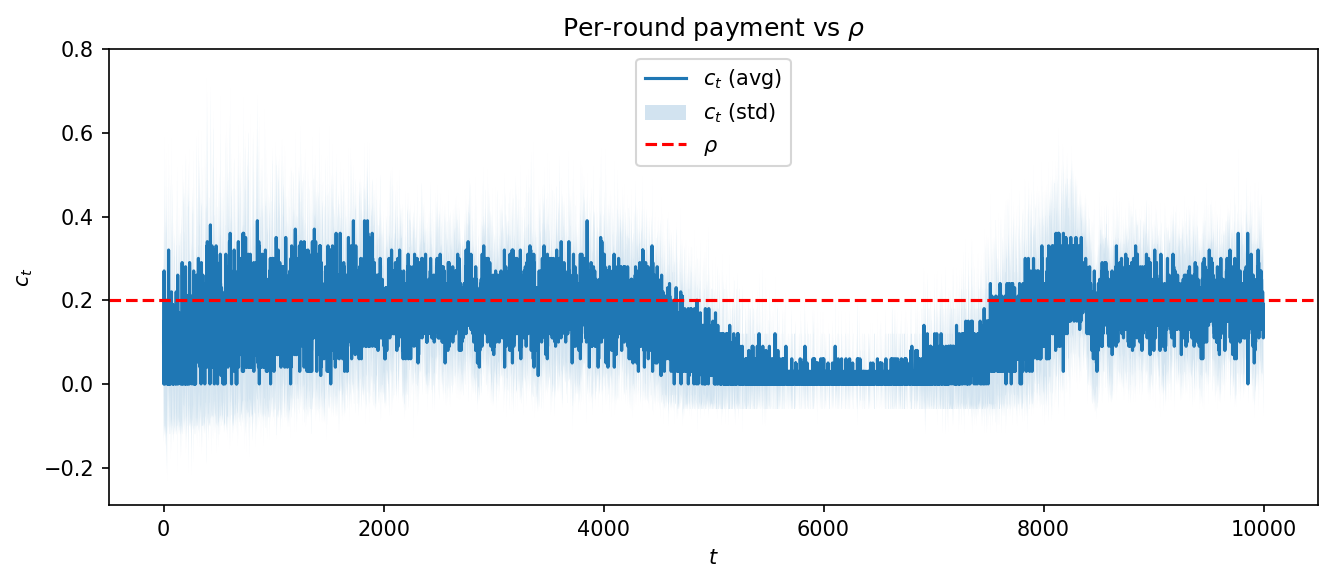
\includegraphics[width=1.1\textwidth]{figures/req3_per_round_payment_vs_rho.png}\\
        \end{column}\hfill
    \end{columns}
     
\end{frame}

% ============================================================
% Results: cumulative regret & payments
% ============================================================
\begin{frame}{Results: primal-dual}
    \begin{columns}[T]
        \begin{column}{0.6\textwidth}
            \centering
            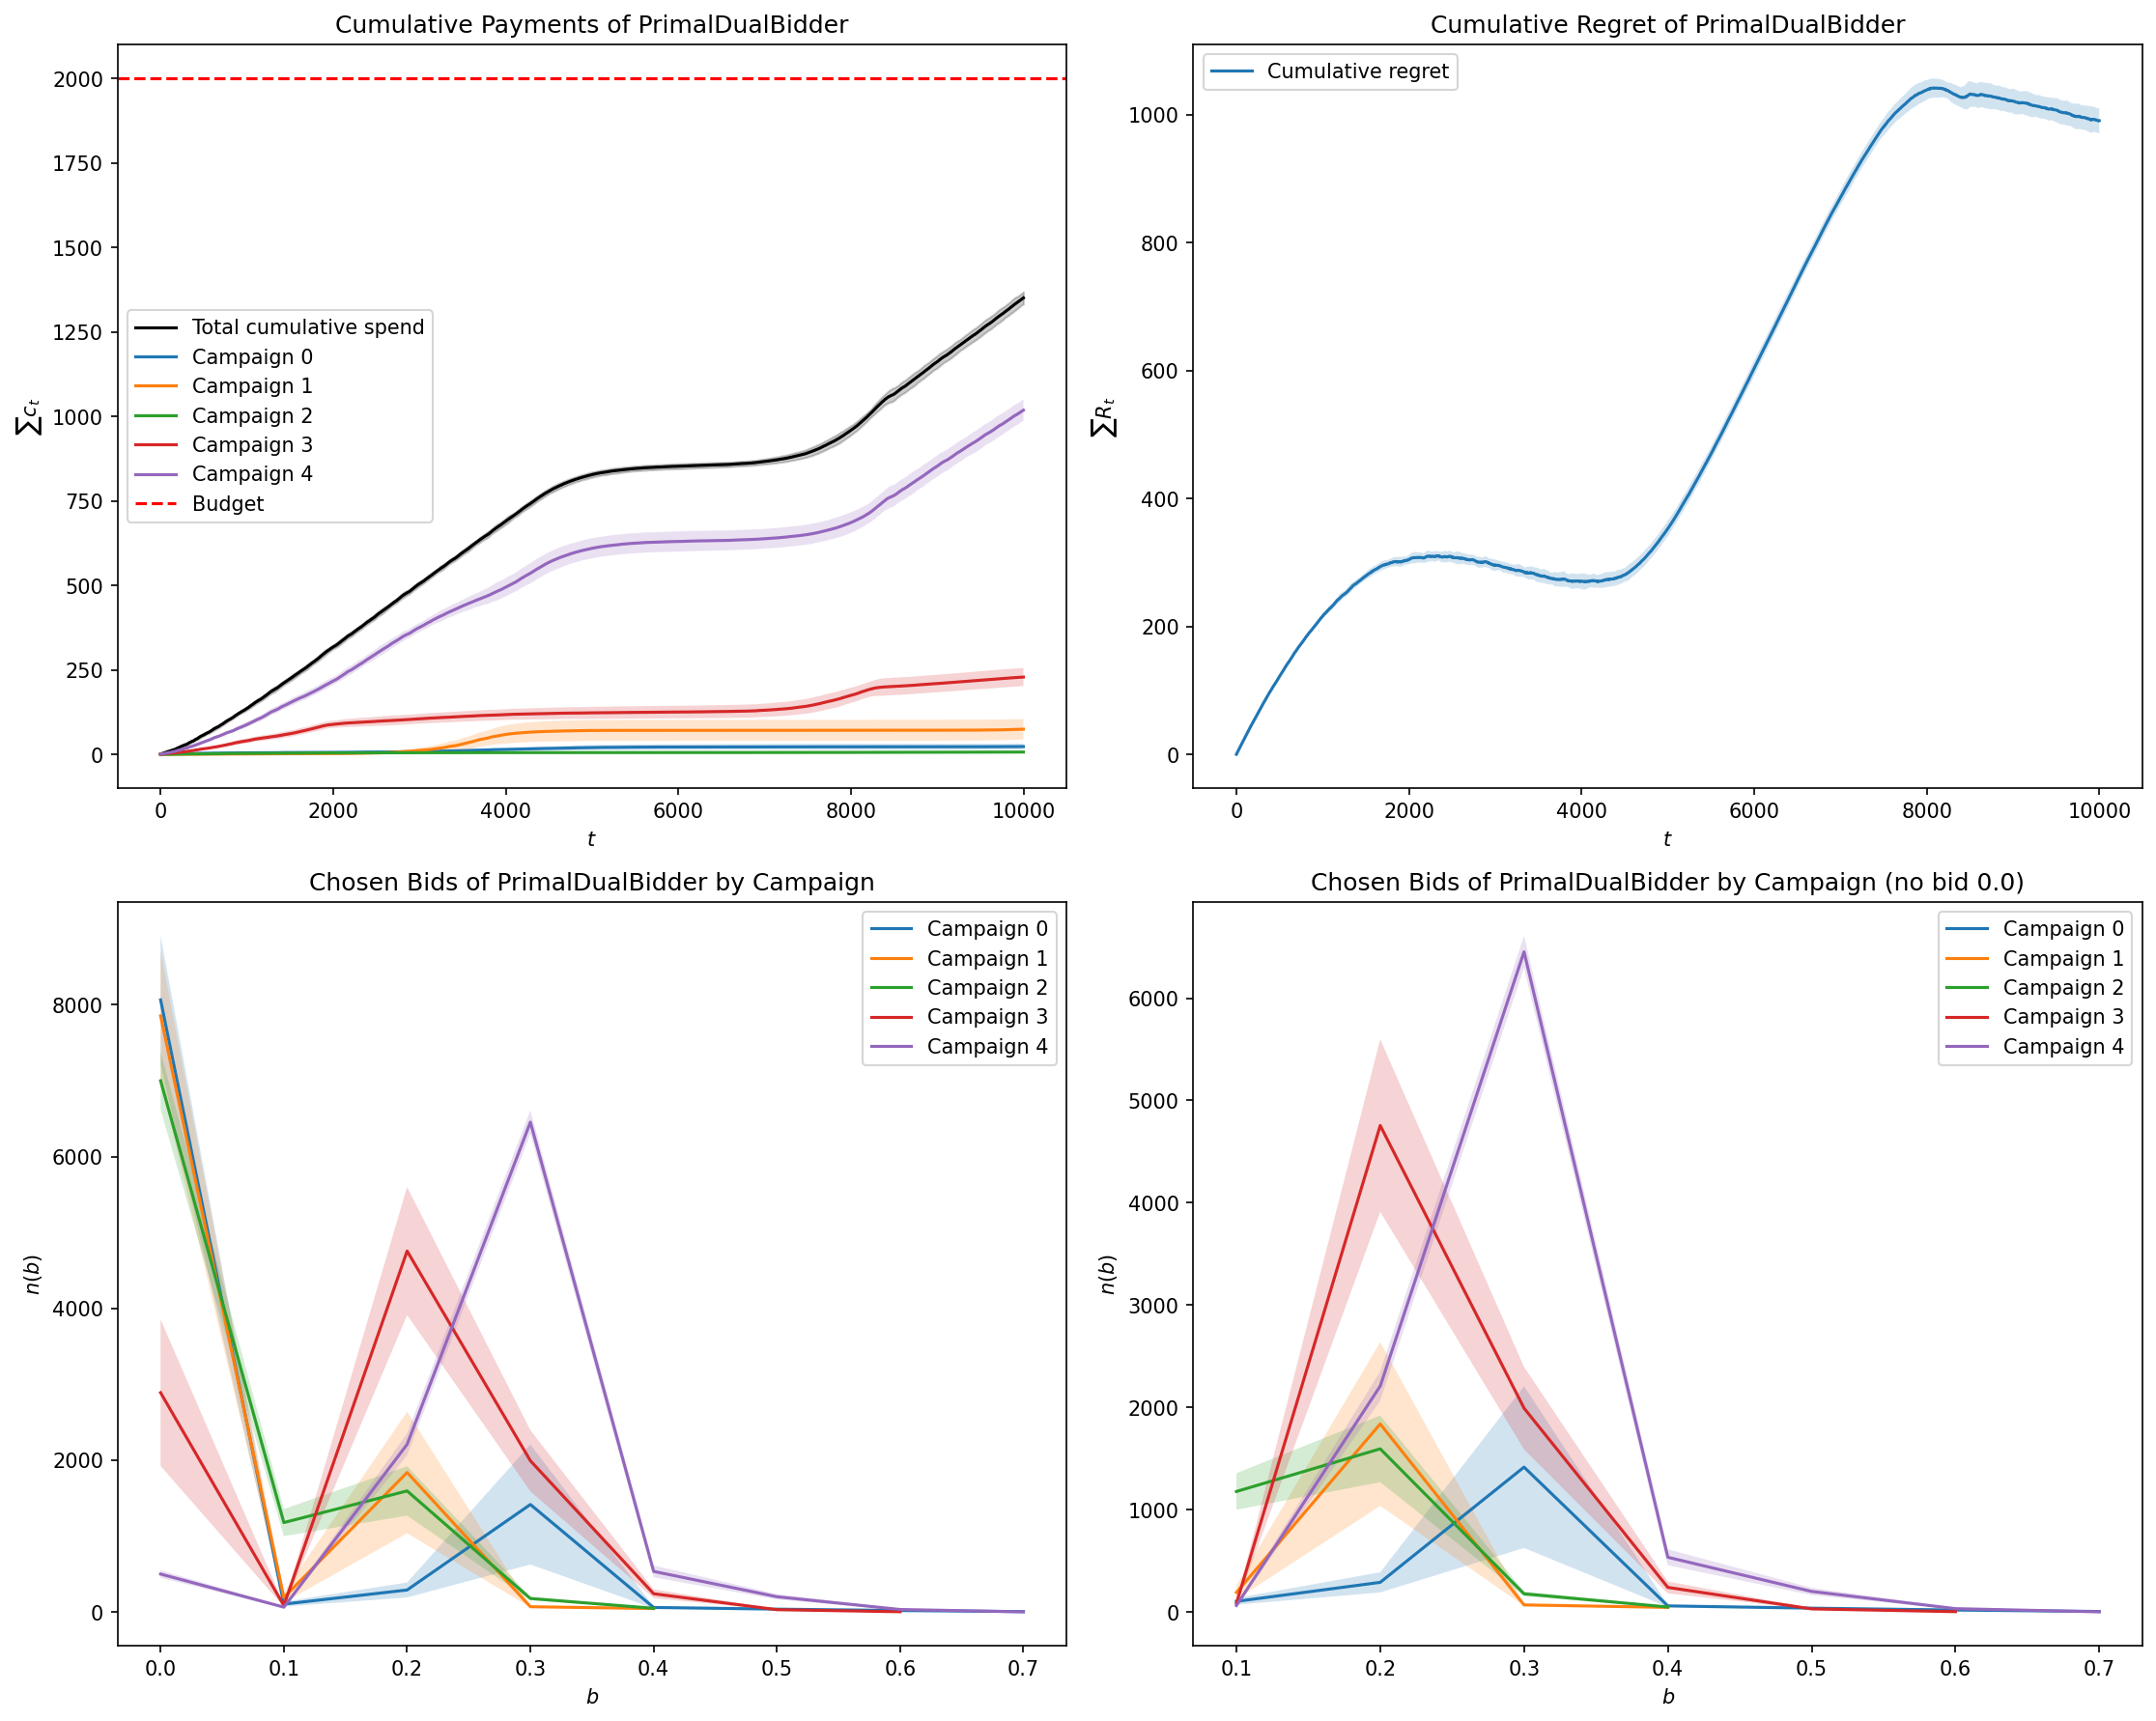
\includegraphics[width=0.9\textwidth]{figures/req3_primal_dual_experiment_results.png}\\
        \end{column}
        \begin{column}{0.4\textwidth}
             \footnotesize\begin{itemize}
                \item The primal-dual bidder is very conservative and spends much less than the budget
                \item This happens whatever the budget is: this bidder never depletes all the budget (observed while making attempts, but not in the notebook)
                \item Regret is sublinear, but clearly follows the trend in the highest competing bids
                \item Bids are (surprisingly) clearly separated: the primal-dual bidder likely acts on the pacing of the bids (how often), not on the value of the bid itself
            \end{itemize}
        \end{column}\hfill
    \end{columns}
\end{frame}